% Numerical Computing II
% Homework 21
% Eigenvalue Computation
% 4/10/2010
% Exercises 21.3, 21.4, 21.5, 21.6, 21.8, 21.12, 21.13

\documentclass[11pt]{article}
\usepackage{listings}
\usepackage[fleqn]{amsmath}
\usepackage{graphicx}
\begin{document}         
% Start your text
\lstset{language=Matlab,numbers=left,frame=single,breaklines=true,morecomment=[l]{//}}
\newcommand{\makehomework}[2]%
{\begin{center}%
	\Huge #1\\%
	\Large #2\\%
	Marty Fuhry\\%
	\today%
\end{center}}
\makehomework{Numerical Computing II}{Homework 21: Eigenvalue Computation}

\section*{Exercise 21.3}



\section*{Exercise 21.4}
% Import Program 
\lstinputlisting{problem_21_4.m}
This program prints out
\begin{flalign*}
    \lambda_1 &= 262.868...\\
    \lambda_2 &= 49.886...\\
    \lambda_3 &= 49.90922...
\end{flalign*}
The $A$ matrix generated has $\lambda_{max}$ = 49.90902.., which is very close to 
the computed eigenvalues from the power method. To get 3 digits of accuracy, we only
needed 3 iterations. After about 12 iterations, the eigenvalues converge completely using
floats in Octave.
\pagebreak
\section*{Exercise 21.5}

The following code was used to generate Table \ref{21.5}.

% Import Program 
\lstinputlisting{problem_21_5.m}

The following is a table of the $n^{th}$ magic matrix's max eigenvalue taken from 
\verb|eig|, and the computed max eigenvalue taken after 10 iterations of the power method.

\begin{table}[h]
    \begin{center}
    \caption{Magic Matrix Eigenvalues}
    \label{21.5}
    \begin{tabular}{| l | c | r|}
        \hline
        $n$ & $\lambda_{max}$ & $\lambda_{computed}$\\
        \hline
        4 & 34 & 33.999...\\
        5 & 65 & 64.999...\\
        6 & 111 & 110.999...\\
        7 & 175 & 174.999...\\
        8 & 260 & 259.999...\\
        9 & 369 & 368.999...\\
            10 & 505 & 505\\
        \hline
        \end{tabular}
    \end{center}
\end{table}

(Note: In this table, '...' denotes a continuation of very similar numbers to the actual value,
not an infinite series or something.)

We get very fast convergence. Trying this with only one iteration also yeilds some very close 
values. Also note that for large values of $n$ (around 100), we still have very good 
convergences. 

Curiously enough, by adding the diagonals 
of each magic matrix, we can quickly find the largest eigenvalue of that matrix. I won't
prove why this is true, or even claim it is; I'll just leave it as a curious observation.
I'll also note that each of the matrices seems to have only eigenvalues with real parts, which is 
curious since they aren't symmetric. Perhaps it's because each matrix is always positive
for each entry.

\section*{Exercise 21.6}

The following code will create a 2000$\times$2000 Toeplitz matrix with 2 on the diagonal and -1
on the super and sub diagonal. It will then start with two random vectors and orthogonalize them.
It will iterate 10 times through subspace iteration and store the two largest eigenvalues in the
\verb|lambda| vector (instead of a matrix).

% Import Program 
\lstinputlisting{problem_21_6.m}

Our results are
\begin{flalign*}
    \lambda_1 &= 3.89740164846829\\
    \lambda_2 &= 3.88879644991644.
\end{flalign*}
Compare these two values with the true values:
\begin{flalign*}
    \lambda_1^* &= 3.99999014026591 \\
    \lambda_2^* &= 3.99999753506496.
\end{flalign*}

Our results are pretty decent after only 10 iterations. After 100 iterations, we get values not much
closer. After 100 iterations, we get
\begin{flalign*}
    \lambda_1 &= 3.98990851058897\\
    \lambda_2 &= 3.98900545116917.
\end{flalign*}

So our subspace iteration was good, but doesn't converge as nicely (or as quickly) as our other examples.

\section*{Exercise 21.8}



\section*{Exercise 21.12}
\section*{Exercise 21.13}
% Import Program 
%\lstinputlisting{problem_17_1.m}

% Import Graph
%\begin{center}
%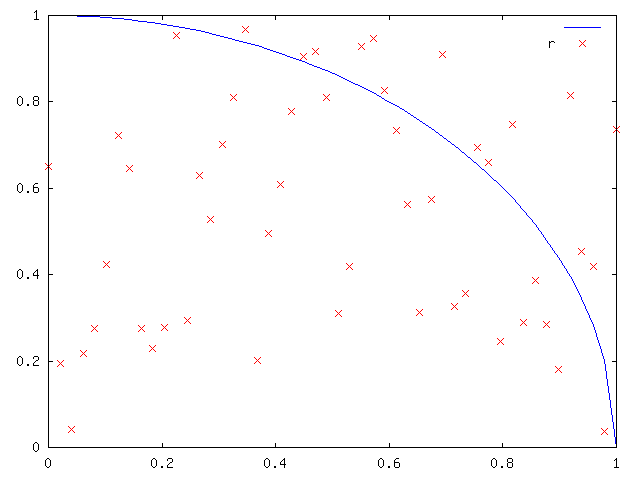
\includegraphics[scale=0.5]{problem_17_1_graph.png}
%\end{center}

% Stop your text
\end{document}
